
\subsection{滤过 $A_\infty$ 同伦的构造 III：同伦的同伦之几何实现}
\label{subsec:7-2-13}

本小节利用第 7.2.10、7.2.12 小节的结果，
完成定理~\ref{thm:4-6-25} 的证明。
为此，要从几何情形（情形~\ref{sit:7-2-263}）
出发，实现定义~\ref{def:7-2-204} 的代数情形。
关键是下述命题~\ref{prop:7-2-275}：
粗略地说，辛微分同胚的“同伦的同伦”
会诱导滤过 $A_{n,K}$ 同态的“同伦的同伦”，
更具体地，诱导定义~\ref{def:7-2-204}
所要求的同伦之间的交换误差同伦 $\mathfrak H_i$。

先描述所用几何情形。
以下使用两个区间 $[0,1]$ 的副本，
分别用 $r$、$s$ 参数化，记为
$[0,1]_r$、$[0,1]_s$。

\begin{statement}{情形}{7.2.263}\label{sit:7-2-263}
设 $(M_0,L_0)$、$(M_1,L_1)$、
$(M'_0,L'_0)$、$(M'_1,L'_1)$
是辛流形与其中相对 spin 的拉格朗日子流形之配对。
设 $\{\psi_{i,s}\}_s$（$i=0,1$）
为第 4.6.2 小节中以 $s\in[0,1]_s$
为参数的两族辛微分同胚
\[
\psi_{i,s}\colon(M_i,L_i)\longrightarrow(M'_i,L'_i),
\]
并设
\begin{equation}
\phi\colon(M_0,L_0)\longrightarrow(M_1,L_1),
\qquad
\phi'\colon(M'_0,L'_0)\longrightarrow(M'_1,L'_1)
\tag{7.2.264}\label{eq:7-2-264}
\end{equation}
也是辛微分同胚。
假定存在以 $(r,s)\in[0,1]_r\times[0,1]_s$
为参数的双参数辛微分同胚族
\begin{equation}
\Phi_{r,s}\colon(M_0,L_0)\longrightarrow(M'_1,L'_1),
\tag{7.2.265}\label{eq:7-2-265}
\end{equation}
使得
\begin{equation}
\Phi_{0,s}=\phi'\circ\psi_{0,s},
\qquad
\Phi_{1,s}=\psi_{1,s}\circ\phi.
\tag{7.2.266}\label{eq:7-2-266}
\end{equation}
\end{statement}

命题~\ref{prop:7-2-275} 表明，
在情形~\ref{sit:7-2-263} 下，
可构造满足定理~\ref{thm:7-2-212}
前提的滤过 $A_{n,K}$ 代数及同态。

\begin{remark}{7.2.267}\label{rem:7-2-267}
实际上，证明定理~\ref{thm:4-6-25}
只用到
$(M_0,L_0)=(M_1,L_1)$、
$(M'_0,L'_0)=(M'_1,L'_1)$，
以及 $\phi=\operatorname{id}$、
$\phi'=\operatorname{id}$ 的情形。
不过，在情形~\ref{sit:7-2-263}
这一更一般的框架中，
论证的基本思想较易看清。
\end{remark}

我们的主要任务是从几何的
$\{\Phi_{r,s}\}_{r,s}$
构造代数的“同伦的同伦”。
在开始之前，回顾第 7.2.9、7.2.10 小节
构造的若干滤过 $A_{n,K}$ 同态与同伦。

取实数 $\lambda_0,\lambda_1,\lambda'_0,\lambda'_1$，
使
$\lambda_0<\lambda_1\le\lambda'_1$、
$\lambda_0\le\lambda'_0<\lambda'_1$。
给定 $\phi$（相应地 $\phi'$），
可配以滤过
$A_{n'(\lambda_0),K'(\lambda_0)}$
（相应地
$A_{n'(\lambda'_0),K'(\lambda'_0)}$）
同态
\begin{equation}
\mathfrak f^\phi\colon
C(L_0,\lambda_0)\longrightarrow
C(L_1,(\lambda_0,\lambda_1)),
\tag{7.2.268.1}\label{eq:7-2-268-1}
\end{equation}
\begin{equation}
\mathfrak f^{\phi'}\colon
C(L'_0,\lambda'_0)\longrightarrow
C(L'_1,(\lambda'_0,\lambda'_1)).
\tag{7.2.268.2}\label{eq:7-2-268-2}
\end{equation}
定义 (7.2.268.1)--(7.2.268.2)
需要选定（或选定一族）殆复结构、多值截面及子复形。
此前各小节已多次把这些选取纳入
滤过 $A_{n,K}$ 同态和运算的记号；
本小节不再写出这些附加记号。
把 (7.2.268) 与包含映射的同伦逆复合，得
\begin{equation}
\mathfrak g^\phi\colon
C(L_0,\lambda_0)\longrightarrow C(L_1,\lambda_1),
\tag{7.2.269.1}\label{eq:7-2-269-1}
\end{equation}
\begin{equation}
\mathfrak g^{\phi'}\colon
C(L'_0,\lambda'_0)\longrightarrow C(L'_1,\lambda'_1).
\tag{7.2.269.2}\label{eq:7-2-269-2}
\end{equation}
同样，$\psi_{i,s_0}$（$i=0,1$，
$s_0=0,1$）诱导
\begin{equation}
\mathfrak f^{\psi_{i,s_0}}\colon
C(L_i,\lambda_i)\longrightarrow
C^{s=s_0}(L'_i,(\lambda_i,\lambda'_i)),
\tag{7.2.270}\label{eq:7-2-270}
\end{equation}
\begin{equation}
\mathfrak g^{\psi_{i,s_0}}\colon
C(L_i,\lambda_i)\longrightarrow C(L'_i,\lambda'_i).
\tag{7.2.271}\label{eq:7-2-271}
\end{equation}

同伦 $\{\psi_{i,s}\}_s$
确定滤过 $A_{n''(\lambda'_i),k''(\lambda'_i)}$ 代数
\[
C([0,1]_s\times L'_i,(\lambda_i,\lambda'_i))
\]
及同阶滤过映射
\begin{equation}
\operatorname{Incl}_s\colon C(L'_i,\lambda'_i)
\longrightarrow
C([0,1]_s\times L'_i,(\lambda_i,\lambda'_i)),
\tag{7.2.272.1}\label{eq:7-2-272-1}
\end{equation}
\begin{equation}
\operatorname{Eval}_{s=s_0}\colon
C([0,1]_s\times L'_i,(\lambda_i,\lambda'_i))
\longrightarrow
C^{s=s_0}(L'_i,(\lambda_i,\lambda'_i)).
\tag{7.2.272.2}\label{eq:7-2-272-2}
\end{equation}
其中 $\operatorname{Incl}$、
$\operatorname{Eval}$ 满足 (7.2.175)。
另有滤过
$A_{n''(\lambda_i),k''(\lambda_i)}$
同态
\[
\mathfrak f^{\{\psi_{i,s}\}_s}\colon
C(L_i,\lambda_i)\longrightarrow
C([0,1]_s\times L'_i,(\lambda_i,\lambda'_i)),
\]
满足
\begin{equation}
\operatorname{Eval}_{s=s_0}
\circ\mathfrak f^{\{\psi_{i,s}\}_s}
=\mathfrak f^{\psi_{i,s_0}}.
\tag{7.2.273}\label{eq:7-2-273}
\end{equation}

设 $\mathfrak C'_0$ 是
$[0,1]_s\times C(L'_0,\lambda'_0)$
的一个模型。
由定理~\ref{thm:7-2-176}，
可构造
\begin{equation}
\mathfrak j_{[0,1]_s}\colon
C([0,1]_s\times L'_0,(\lambda_0,\lambda'_0))
\longrightarrow\mathfrak C'_0,
\tag{7.2.274}\label{eq:7-2-274}
\end{equation}
使图式~\ref{diag:7-2-10}、
\ref{diag:7-2-11} 交换。

\par\medskip\noindent\begin{minipage}{\textwidth}
\centering
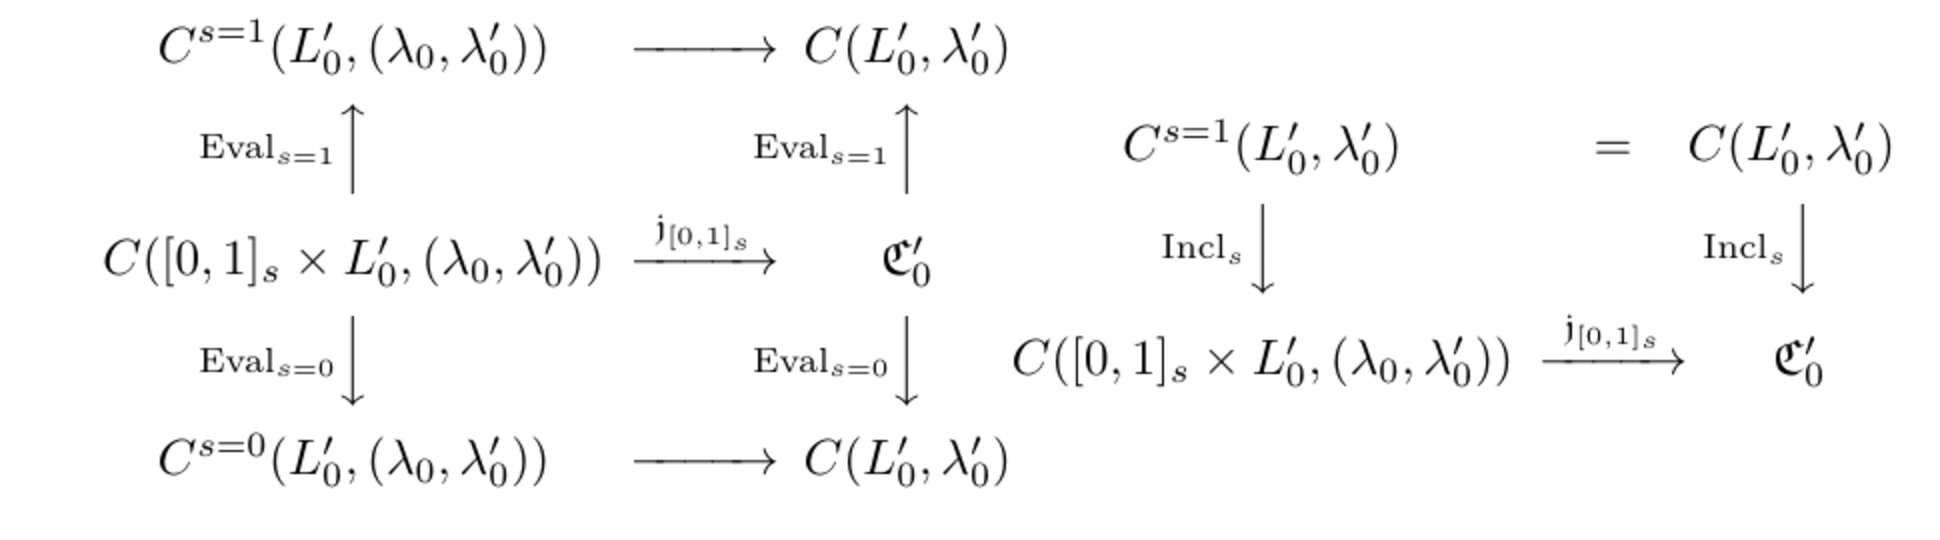
\includegraphics[width=\textwidth]{chapters/ch07-transversality/figures/phys-544-diagram-7-2-10-11-math-crop.png}
\par\noindent
\begin{minipage}{.50\textwidth}\centering
{\renewcommand{\thefigure}{7.2.10}\refstepcounter{figure}
\normalfont\bfseries 图式~\thefigure\label{diag:7-2-10}}
\end{minipage}%
\begin{minipage}{.50\textwidth}\centering
{\renewcommand{\thefigure}{7.2.11}\refstepcounter{figure}
\normalfont\bfseries 图式~\thefigure\label{diag:7-2-11}}
\end{minipage}
\end{minipage}\par\medskip

图式~\ref{diag:7-2-10} 的下行映射是
包含映射的同伦逆。
映射 $\mathfrak j_{[0,1]_s}$
将在引理 7.2.304 中定义。
把 $\mathfrak f^{\{\psi_{0,s}\}_s}$
与 (7.2.274) 复合，得
\[
\mathfrak g^{\{\psi_{0,s}\}_s}
=\mathfrak j_{[0,1]_s}\circ
\mathfrak f^{\{\psi_{0,s}\}_s},
\]
于是图式~\ref{diag:7-2-12} 交换。
设 $\mathfrak C'_1$ 是
$[0,1]_s\times C(L'_1,\lambda'_1)$
的模型。类似地得到
$\mathfrak g^{\{\psi_{1,s}\}_s}$，
使图式~\ref{diag:7-2-13} 交换。

\par\medskip\noindent\begin{minipage}{\textwidth}
\centering
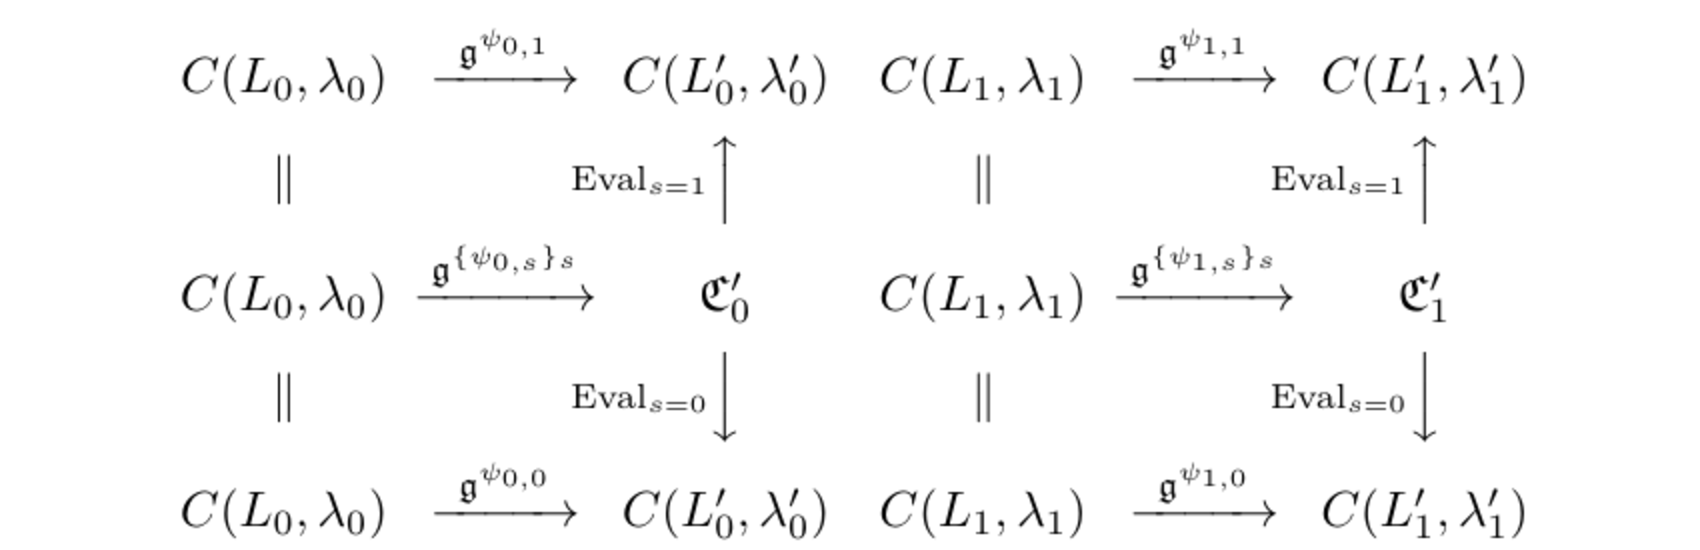
\includegraphics[width=.94\textwidth]{chapters/ch07-transversality/figures/phys-545-diagram-7-2-12-13-math2-crop.png}
\par\noindent
\begin{minipage}{.50\textwidth}\centering
{\renewcommand{\thefigure}{7.2.12}\refstepcounter{figure}
\normalfont\bfseries 图式~\thefigure\label{diag:7-2-12}}
\end{minipage}%
\begin{minipage}{.50\textwidth}\centering
{\renewcommand{\thefigure}{7.2.13}\refstepcounter{figure}
\normalfont\bfseries 图式~\thefigure\label{diag:7-2-13}}
\end{minipage}
\end{minipage}\par\medskip

接下来考察同伦
$\{\Phi_{r,s_0}\}_r$（固定 $s_0=0$ 或 $1$）。
它诱导从
$\mathfrak g^{\phi'}\circ
\mathfrak g^{\psi_{0,s_0}}$
到
$\mathfrak g^{\psi_{1,s_0}}\circ
\mathfrak g^\phi$
的同伦；下面作进一步说明。
设 $\mathfrak C_1'^{(s=s_0)}$
是 $[0,1]\times C(L'_1,\lambda'_1)$
的模型。
存在滤过
$A_{n''(\lambda_0),K''(\lambda_0)}$
同态
\[
\mathfrak g_+^{\{\Phi_{r,s_0}\}_r}\colon
C(L_0,\lambda_0)\longrightarrow
\mathfrak C_1'^{(s=s_0)},
\]
使图式~\ref{diag:7-2-14} 交换；
同时使用图式~\ref{diag:7-2-15}。

\par\medskip\noindent\begin{minipage}{\textwidth}
\centering
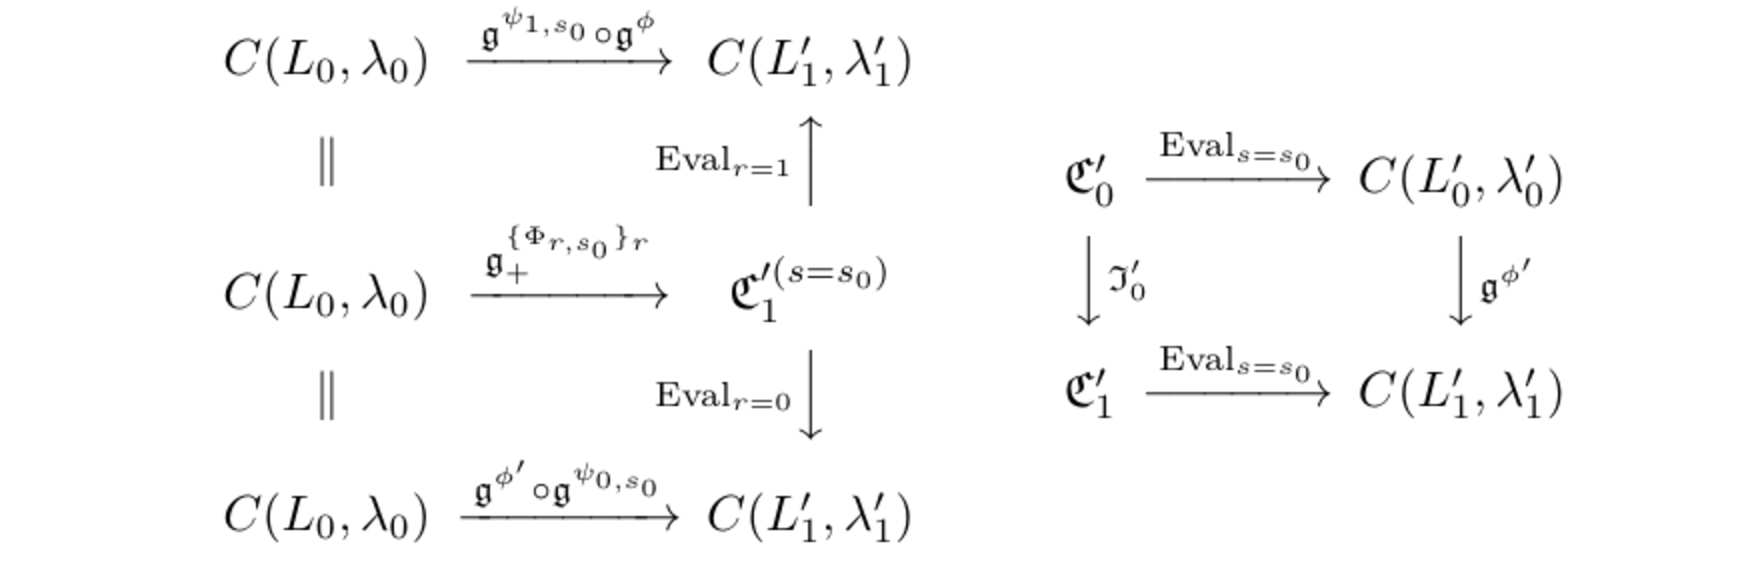
\includegraphics[width=.94\textwidth]{chapters/ch07-transversality/figures/phys-545-diagram-7-2-14-15-math2-crop.png}
\par\noindent
\begin{minipage}{.50\textwidth}\centering
{\renewcommand{\thefigure}{7.2.14}\refstepcounter{figure}
\normalfont\bfseries 图式~\thefigure\label{diag:7-2-14}}
\end{minipage}%
\begin{minipage}{.50\textwidth}\centering
{\renewcommand{\thefigure}{7.2.15}\refstepcounter{figure}
\normalfont\bfseries 图式~\thefigure\label{diag:7-2-15}}
\end{minipage}
\end{minipage}\par\medskip

$\mathfrak g_+^{\{\Phi_{r,s_0}\}_r}$
中下标 $+$ 的缘由，
将在命题~\ref{prop:7-2-275}
的证明中说明。

以下是本小节关于几何“同伦的同伦”
的主要结果\liftIndex{I277}。
\begin{proposition}{7.2.275}\label{prop:7-2-275}
存在 $n'''(\lambda_i)$、$K'''(\lambda_i)$，
满足
\[
\lim_{\lambda_i\to0}n'''(\lambda_i)
=\lim_{\lambda_i\to0}K'''(\lambda_i)=\infty,
\]
并存在
$[0,1]^2\times C(L'_1,\lambda'_1)$
的滤过
$A_{n'''(\lambda'_1),K'''(\lambda'_1)}$
类模型 $\widehat{\mathfrak C}'_1$，
以及滤过
$A_{n'''(\lambda_0),K'''(\lambda_0)}$
同态
$\mathcal I'_0\colon\mathfrak C'_0\to\mathfrak C'_1$
和
\[
\mathfrak H\colon C(L_0,\lambda_0)
\longrightarrow\widehat{\mathfrak C}'_1,
\]
满足：

\par\noindent\textup{(7.2.276.1)}
上面的图式~\ref{diag:7-2-15} 交换。

\par\noindent\textup{(7.2.276.2)}
$\widehat{\mathfrak C}'_{1,r=r_0}
=\mathfrak C'_1$；
此处等号表示它们作为
$[0,1]_s\times C(L'_1,\lambda'_1)$
的 $A_{n'''(\lambda_0),K'''(\lambda_0)}$
类模型相等。

\par\noindent\textup{(7.2.276.3)}
$\widehat{\mathfrak C}'_{1,s=s_0}
=\mathfrak C_1'^{(s=s_0)}$；
此处等号表示它们作为
$[0,1]_r\times C(L'_1,\lambda'_1)$
的同阶模型相等。

\par\noindent\textup{(7.2.276.4)}
$\operatorname{Eval}_{r=0}\circ\mathfrak H
=\mathcal I'_0\circ
\mathfrak g^{\{\psi_{0,s}\}_s}$。

\par\noindent\textup{(7.2.276.5)}
$\operatorname{Eval}_{r=1}\circ\mathfrak H
=\mathfrak g^{\{\psi_{1,s}\}_s}
\circ\mathfrak g^\phi$。

\par\noindent\textup{(7.2.276.6)}
$\operatorname{Eval}_{s=s_0}\circ\mathfrak H
=\mathfrak g_+^{\{\Phi_{r,s_0}\}_r}$。
\end{proposition}

见图式~\ref{diag:7-2-16}。
\par\medskip\noindent\begin{minipage}{\textwidth}
\centering
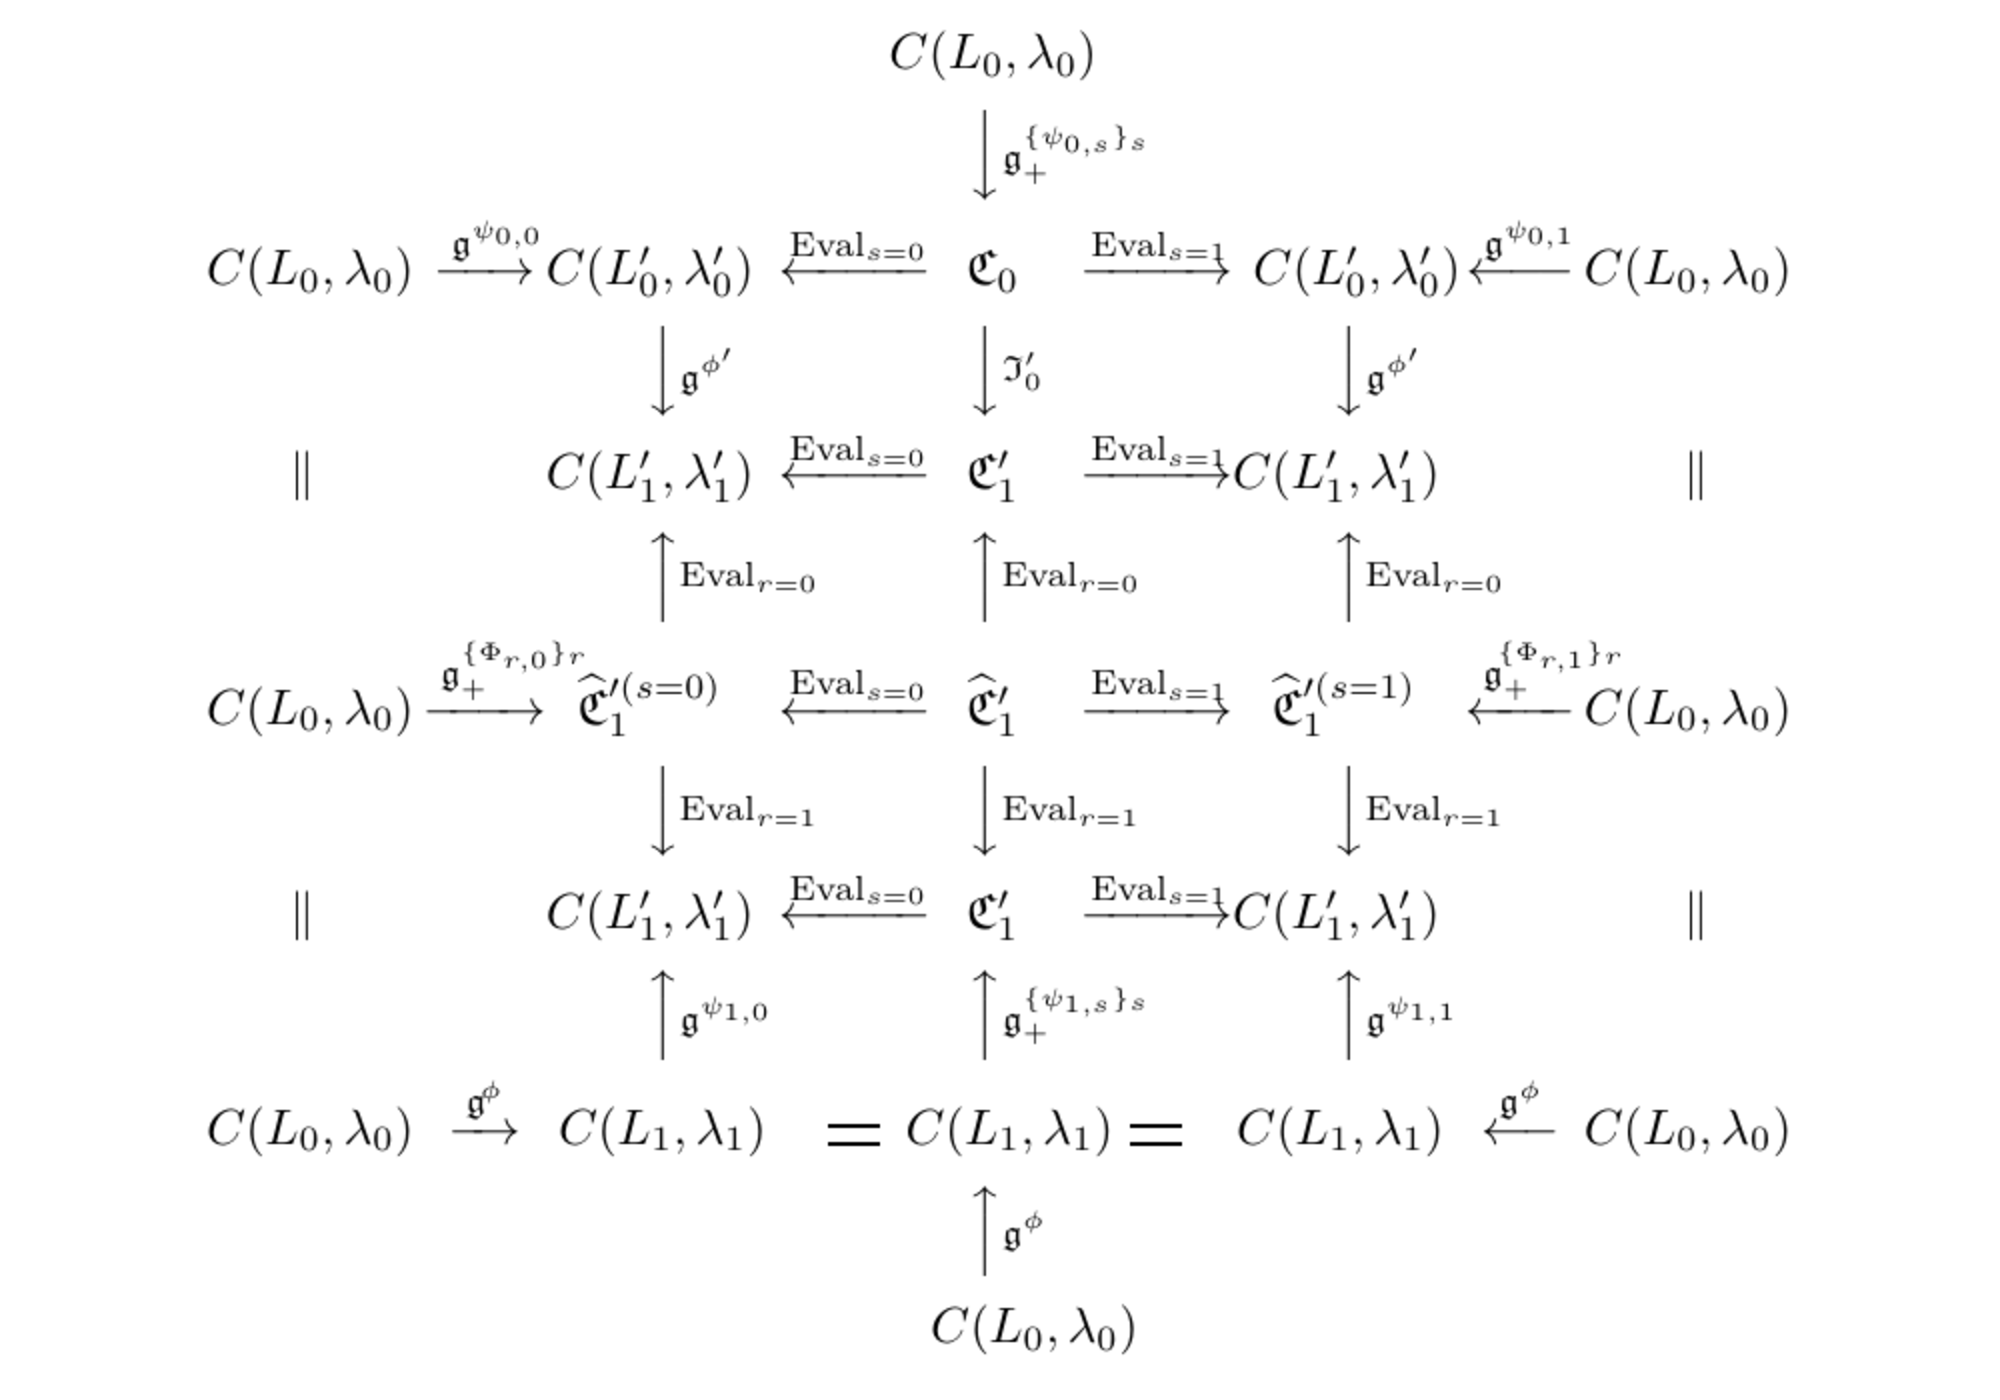
\includegraphics[width=\textwidth]{chapters/ch07-transversality/figures/phys-546-diagram-7-2-16-math-crop.png}
\par{\renewcommand{\thefigure}{7.2.16}\refstepcounter{figure}
\normalfont\bfseries 图式~\thefigure\label{diag:7-2-16}}
\end{minipage}\par\medskip
\noindent\textbf{译者注：}
原书图式~\ref{diag:7-2-16}
在 $\{\psi_{i,s}\}_s$ 对应的箭头上写
$\mathfrak g_+$，
而邻近文字、图式~\ref{diag:7-2-12}--\ref{diag:7-2-13}
及条件 (7.2.276.4)--(7.2.276.5) 写 $\mathfrak g$。
图式保留源书原貌；命题证明中
(7.2.276.4)--(7.2.276.5) 的两条端面计算
均使用 $\mathfrak g$，只有五段复合的中间同伦
使用 $\mathfrak g_+$，故这里的 $+$ 按图式记号误植处理。

下一命题~\ref{prop:7-2-277}
还保证条件 7.2.215 成立。
\begin{proposition}{7.2.277}\label{prop:7-2-277}
存在 $n''''(\lambda_i)$、$K''''(\lambda_i)$，
满足
\[
\lim_{\lambda_i\to0}n''''(\lambda_i)
=\lim_{\lambda_i\to0}K''''(\lambda_i)=\infty,
\]
并存在
$[0,1]^2\times C(L'_1,\lambda'_1)$
的滤过
$A_{n''''(\lambda'_1),K''''(\lambda'_1)}$
类模型 $\widetilde{\mathfrak C}'_1$，
以及滤过
$A_{n''''(\lambda_1),K''''(\lambda_1)}$
同态
\[
\widetilde{\mathfrak H}\colon
C(L'_0,\lambda'_0)\longrightarrow
\widetilde{\mathfrak C}'_1,
\]
满足：

\par\noindent\textup{(7.2.278.1)}
$\widetilde{\mathfrak C}'_{1,r=r_0}
=\mathfrak C'_1$；
此处等号表示它们作为
$[0,1]_s\times C(L'_1,\lambda'_1)$
的 $A_{n''''(\lambda_1),K''''(\lambda_1)}$
类模型相等。

\par\noindent\textup{(7.2.278.2)}
$\operatorname{Eval}_{r=0}\circ\widetilde{\mathfrak H}
=\mathcal I'_0\circ\operatorname{Incl}_s$。

\par\noindent\textup{(7.2.278.3)}
$\operatorname{Eval}_{r=1}\circ\widetilde{\mathfrak H}
=\operatorname{Incl}_s\circ\mathfrak g^{\phi'}$。

\par\noindent\textup{(7.2.278.4)}
$\operatorname{Eval}_{s=s_0}\circ\widetilde{\mathfrak H}
=\operatorname{Incl}_r\circ\mathfrak g^{\phi'}$。
\end{proposition}

\noindent\textbf{译者注：}
原书上述两命题的阶数函数写极限
$\lambda_i\to0$；
但定义~\ref{def:7-2-182} 的有向系统
要求 $\lambda_i\to\infty$，
下面的定理~\ref{thm:4-6-25} 证明
也要将这些阶数函数用于该系统。
这里暂保留源式，极限方向留待证明步骤核查。

在证明命题~\ref{prop:7-2-275}、
\ref{prop:7-2-277} 之前，
先以两命题为前提证明
定理~\ref{thm:4-6-25}。

\par\noindent\textit{定理~\ref{thm:4-6-25} 的证明。}
考虑该定理的情形。
它是情形~\ref{sit:7-2-263} 的特例：
置
\[
\begin{gathered}
(M_0,L_0)=(M_1,L_1)=(M,L),\\
(M'_0,L'_0)=(M'_1,L'_1)=(M',L'),\\
\psi_{i,s}=\psi_s,\qquad
\phi=\phi'=\operatorname{id},\qquad
\Phi_{r,s}=\psi_s .
\end{gathered}
\]
其中右侧记号来自定理~\ref{thm:4-6-25}，
左侧记号来自情形~\ref{sit:7-2-263}。
\translatornote{原书此处把左侧
$\psi_{i,s}$ 写为 $\psi_{r,s}$；
但情形~\ref{sit:7-2-263} 的该族以下标
$i=0,1$ 标识，$r$ 属于双参数族 $\Phi_{r,s}$。
此处依两族的源靶定型。}
又置
\[
\lambda_i=\lambda'_i,\qquad
\bar n(\lambda_i)=n'''(\lambda_i),\qquad
\bar k(\lambda_i)=K'''(\lambda_i),
\]
右侧记号来自命题~\ref{prop:7-2-275}，
左侧来自定理~\ref{thm:7-2-212}。

选取 $\lambda_i,\lambda'_i$，
使下列滤过
$A_{n'(\lambda_i),K'(\lambda_i)}$
同态对 $s_0=0,1$ 均有定义：
\begin{equation}
\mathfrak g^{\psi_{s_0},\lambda_i}\colon
C(L,\lambda_i)\longrightarrow C(L',\lambda'_i).
\tag{7.2.279}\label{eq:7-2-279}
\end{equation}
此外，$\phi=\operatorname{id}$ 诱导
滤过 $A_{n'(\lambda_i),K'(\lambda_i)}$
同态
\[
I_i=\mathfrak h^{\lambda_i,\lambda_{i+1}}\colon
C(L,\lambda_i)\longrightarrow C(L,\lambda_{i+1}),
\]
它正是 $\mathfrak g^\phi$。
同样，$I'_i=\mathfrak g^{\phi'}$，
其中 $\phi'=\operatorname{id}$。
置
\[
\mathcal F_i^{s=s_0}
=\mathfrak g_+^{\{\Phi_{r,s_0}\}_r},
\qquad
\mathcal H_i=\mathfrak g^{\{\psi_s\}_s},
\qquad
C_i=C(L,\lambda_i),\qquad
C'_i=C(L',\lambda'_i).
\]
对每个 $i$，
在命题~\ref{prop:7-2-275} 中取
$\lambda_0=\lambda_i$、
$\lambda_1=\lambda_{i+1}$。
于是定理~\ref{thm:7-2-212}
（即定义~\ref{def:7-2-204}）
的前提得到满足。
注意，在此特例中
$\widehat{\mathfrak C}'_{i,r=0}
=\widehat{\mathfrak C}'_{i,r=1}
=\mathfrak C'_i$。
命题~\ref{prop:7-2-277}
还保证条件 7.2.215。
因此定理~\ref{thm:4-6-25}
由推论~\ref{cor:7-2-219} 得证。\hfill$\square$
